\documentclass[a4paper,fleqn,usenatbib]{mnras}

%=========================================================================
\usepackage{amsmath} 
\usepackage{amssymb} 
\usepackage{graphicx}
\usepackage{grffile}
\usepackage[dvips]{epsfig}
\usepackage{epsfig}  
\usepackage{color}
\usepackage{caption}
\usepackage{hyperref}
\usepackage{bm}
%Non reposionated tables




%=========================================================================
%		INTERNAL MACROS
%=========================================================================
\def\be{\begin{equation}}
\def\ee{\end{equation}}
\def\ba{\begin{eqnarray}}
\def\ea{\end{eqnarray}}

% To highlight comments 
\definecolor{red}{rgb}{1,0.0,0.0}
\newcommand{\red}{\color{red}}
\definecolor{darkgreen}{rgb}{0.0,0.5,0.0}
\newcommand{\SRK}[1]{\textcolor{darkgreen}{\bf SRK: \textit{#1}}}
\newcommand{\SRKED}[1]{\textcolor{darkgreen}{\bf #1}}
\newcommand{\before}[1]{\textcolor{red}{ #1}}
\newcommand{\after}[1]{\textcolor{darkgreen}{ #1}}
\newcommand{\hs}{{\hspace{1mm}}}  
\newcommand{\tol}{Tololo 1214-277}
\newcommand{\HI}{{\text{H\MakeUppercase{\romannumeral 1}}} }
\newcommand{\HII}{{\text{H\MakeUppercase{\romannumeral 2}}} }
\newcommand{\lya}{\ifmmode{{\rm Ly}\alpha}\else Ly$\alpha$\ \fi}
\newcommand{\cm}{\ifmmode{{\rm cm}}\else cm\fi}
\newcommand{\ccm}{\,\mathrm{cm}^{-3}}
\newcommand{\ergps}{\,{\rm erg}\,{\rm s}\ifmmode{}^{-1}\else ${}^{-1}$\fi}
\newcommand{\Mpch}{\,{\rm Mpc}\,\ifmmode h^{-1}\else $h^{-1}$\fi}
\newcommand{\dd}{\mathrm{d}}
\newcommand{\vek}[1]{\bm{#1}}
\newcommand{\hb}{H$\beta$}
\newcommand{\ha}{H$\alpha$}
\newcommand{\oiii}{[OIII]}
\newcommand{\oii}{[OII]}
\newcommand{\nii}{[NII]}
\newcommand{\esca}{erg cm$^{-2}$ s$^{-1}$ \AA$^{-1}$}
\newcommand{\esc}{erg cm$^{-2}$ s$^{-1}$}
\newcommand{\es}{erg s$^{-1}$}
\newcommand{\esa}{erg s$^{-1}$}
\newcommand{\kms}{\ifmmode\mathrm{km\ s}^{-1}\else km s$^{-1}$\fi}
\newcommand{\hMsun}{{\ifmmode{h^{-1}{\rm{M_{\odot}}}}\else{$h^{-1}{\rm{M_{\odot}}}$}\fi}}
\newcommand{\Msun}{{\ifmmode{{\rm{M_{\odot}}}}\else{${\rm{M_{\odot}}}$}\fi}}

\newcommand{\jefr}[1]{\textcolor{darkgreen}{\bf JEFR: \textit{#1}}}

\begin{document}

%=========================================================================
%		FRONT MATTER
%=========================================================================
\title[Satellites in the MW and M31]{Local Group Satellite Distributions in
 the Illustris Simulation}
\author[J.E. Forero-Romero \& V. Arias]
{Jaime E. Forero-Romero $^{1}$ \thanks{je.forero@uniandes.edu.co},
Ver\'onica Arias$^1$\\
%%
$^1$ Departamento de F\'isica, Universidad de los Andes, Cra. 1
  No. 18A-10 Edificio Ip, CP 111711, Bogot\'a, Colombia \\
}

\maketitle

\begin{abstract}
We quantify the joint spatial distribution of satellites around the Milky way and Andromeda.
\end{abstract}

\begin{keywords}Galaxies: halos --- Galaxies: high-redshift --- Galaxies: statistics
--- Dark Matter --- Methods: numerical 
\end{keywords}

\section{Introduction}

\section{Observational Data}
\label{sec:obs}


\section{Local Group Satellites in the Illustris Simulation}
\label{sec:NumericalSetup}

We use publicly available data from the Illustris Project 
\citep{2014MNRAS.444.1518V}. 
This suite of cosmological simulations, performed using the quasi-Lagrangian
code AREPO \citep{2010MNRAS.401..791S}, followed the coupled evolution of dark 
matter and gas and includes parametrizations to account for the effects of
gas cooling, photoionization, star formation, stellar feedback, black
hole and super massive black hole feedback. 
The simulation volume is a cubic box of $75$ \Mpch\ on a side.
The cosmological parameters correspond to a $\Lambda$CDM cosmology
consistent with WMAP-9 measurements \citep{2013ApJS..208...19H}. 

We extract halo and galaxy information from the Illustris-1 simulation
which has the highest resolution in the current release of the
Illustris Project.
Illustris-1 has $1820^3$ dark matter particles and $1820^3$ initial gas
volumen elements. 
This corresponds to a dark matter particle mass of
$6.3\times 10^6$\Msun\ and a minimum mass for the baryonic volume
element of $8.0\times 10^7$\Msun. 
The corresponding spatial resolution is $1.4$ kpc for the dark matter
gravitational softening and $0.7$ kpc for the typical size of the
smallest gas cell size. 

The smallest satellites are barely resolved in stellar mass at magnitudes of
$M_V=9$, however its dark matter structure is sampled with at least
$100$ particles. 
We find that all considered halos have at least $XX$ subhalos above
a maximum circular velocity of $15$\kms.
For this reason we select the satellite galaxy samples from the
DM subhalo population and not from the galaxies with photometry.
We chose in two different ways the sub-halo samples. 
First, we rank the halos by decreasing order of its maximum circular
velocity and select the first $N_p$ halos in the list.
Second, we select all satellites above maximum circular velocity of
$20$\kms to randmbly subsample $N_p$ subhalos.


We build a sample of Local Group Analgues (LGA) by selecting first all
galaxies with  an stellar mass in the range $1\times10^{10}\Msun
<M_{\star}<1.5 \times 10^{11} \Msun$.
Then we consider the following criteria for all galaxies in that
sample.

\begin{itemize}
\item For each galaxy $A$ we find its closest galaxy $B$, if galaxy $A$ is also
the closest to halo $B$, the two are considered as a pair. 
\item With $d_{AB}$ the distance between the two galaxies and
  $M_{\star,min}$ the lowest stellar mass in the two galaxies, we
  discard pairs that have any other galaxy $C$ with stellar mas
  $M_{\star}>M_{\star, min}$ closer than $3\times d_{AB}$ from any of
  the pair's members. 
\item The distance $d_{AB}$ greater than $700$ kpc.
\item The relative radial velocity between the two galaxies, including
  the Hubble flow, is $-120\ \kms <v_{AB,r}<0\ \kms$. 
\end{itemize}

We find 27 pairs with these conditions. Figure shows the physical 
properties (stellar masses, maximum circular velocities, radial
velocities and separation) in those pairs. 




\section{Satellite Spatial Distribution}
\label{sec:SpatialMeasurements}

We base all our results on the description provide by the inertia
tensor defined by the satellites's positions.  

\begin{equation}
{\bf{\bar{I}}} = \sum_{k \in V}[(\bf{r}_i - \bf{r}_0)^2\cdot \bf{1} -
  (\bf{r}_i-\bf{r}_0)\cdot (\bf{r}_i - \bf{r}_0)^{T}],
\end{equation}
%
where $k$ indexes the set of satellites of interest
$\bf{r}_k$ are the satellites' positions, $\bf{r}_{0}$ is the location
of the satelites's geometric center ${\bf r}_{0}\equiv \frac{1}{N_s}\sum_{k\in
  V} \bf{r}_i$, $\bf{1}$ is the unit matrix,  and  
${\bf r}^T$ is the transposed vector $\bf{r}$. 

From this tensor we compute its eigenvalues,
$\lambda_1>\lambda_2>\lambda_3$, and corresponding eigenvectors,
$\hat{I}_1$, $\hat{I}_2$, $\hat{I}_3$.
We define the size of its three ellipsoidal axis as
$a=\sqrt{\lambda_1}$, $b=\sqrt{\lambda_2}$ and $c=\sqrt{\lambda_3}$.

We define $\hat{n}\equiv \hat{I}_1$ as the vector perpendicular to the
planar satellite distribution. 
We also define the width of the planar satellite distribution,
$\sigma_p$ as the standard deviation of all satellite distances to the
plane defined by the $\hat{n}$.

We characterize the alignment between the satellite plane and the
vector connecting the two dominant galaxies as $\mu=|\hat{r}_{AB}\cdot
\hat{n}|$. 
It has been shown that LG pair separation vector is aligned along the
filaments in  which they are typically embeded
\cite{2015ApJ...799...45F}, the LG pairs found in pancake-like DM
matter arrangements are aligned with the plane itself. 
Characterizing the satellite alignments with $\mu$ thus provide
information about how satellites are distributed with respect to the
cosmic web. 

\subsection{Parameter Distributions}

We charaterize the $\mu$ distribution by a power law probability
density distribution
\begin{equation}
P(\mu) = \frac{1}{\alpha}\mu^{\alpha-1}.
\end{equation}
We estimate the $\alpha$ using a bayesian approach, such as that
the likelihood of being $\alpha$ the power value given the observed values of $\{\mu_i\}$
  can be written as:

\begin{equation}
\mathcal{L}(\alpha|\{\mu_i\})=\frac{1}{Z_\alpha}\prod_{i=1}^{N_s}
\frac{1}{\alpha}\mu_i^{\alpha-1}, 
\end{equation}
%
where $Z_{\alpha}$ is a constant such as $\int_{0}^{\infty}
{\mathcal L}(\alpha|\{\mu_i\}) {\rm d}\alpha=1$. 
We report as $\hat{\alpha}$ the value of $\alpha$ 
maximizing the likelihood,

We characterize the distributions for the plane width and axis ratio
$b/a$, $b/c$ through a gaussian
\begin{equation}
P(x)  = \frac{1}{\sqrt{2\pi \sigma^2}} \exp{\left[-\frac{1}{2}\left(\frac{x-x_m}{\sigma}\right)^2\right]}
\end{equation}
In this case the maximum likelihood values for the parameter estimates
$\hat{x_m}$ and $\hat{\sigma}$ correspond to the mean and standard
deviation, respectively.

We summarize the results from the Illustris simulation by reporting
the maximum likelihood parameter estimates. 
In turn we use this us to estimate the probability of finding the
observed values in the Local Group and compare it against the highest
probabilty values.


\subsection{Satellite samples}

We compare the satellite distributions in the MW and M31 at fixed
satellite number.
This means that the magnitude cut corresponding to the faintest
satellite included in the sample is different in each case.
We make this choice for two reasons. 
First to always be sure that there is a non-zero number of satellites to make the computations. 
Second, to be able to compare the two halos at a fixed number of
satellites. 

We test the shape and alignment statistics for 11 up 15 satellites.
The lowest number corresponds to the number of classical Milky Way
satellites.
The upper limit corresponds to the minimum number of satellites that
can be resolved in the simulations for both halos in each pair. 
In the case of simulations we rank the subhalos by their maximum
circular velocity. 
We do not use their stellar properties because this represents the
lower resolution limit for the hydrodynamics; most of these subhalos
only have one stellar particle belonging to them. 
In contrast, the detected sub-halos have at least 35 dark matter
particles to determine their properties.


We build two different kinds of statistics from these satellites
First, we compute the shape and alignments for a varying number of
satellites $11\leq N_{s}\leq 15$ keeping their ranking in
$M_V$ or $V_{max}$. 
This allows us to estimate the variation expected by changing the
satellite number. 
The second kind of statistics are computed for a fixed number of
satellites $N_{s}=11$ randomly selected from the top $15$ ranked
satellites. 
We perform this bootstrapping $10$ times for each pair. 
This allows us to estimate the variation expected by randomly sampling
the satellites from a parent distribution.





% referencia posiciones satellites
% http://adsabs.harvard.edu/abs/2013MNRAS.435.1928P

\begin{figure*}
\centering
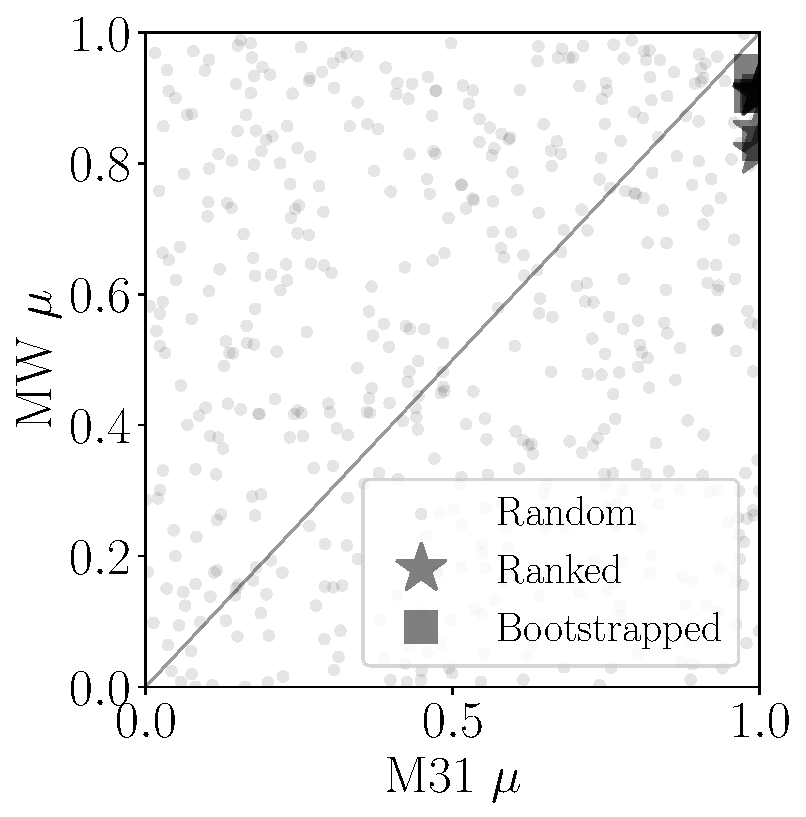
\includegraphics[width=0.40\textwidth]{LG_scatter_mu.pdf}
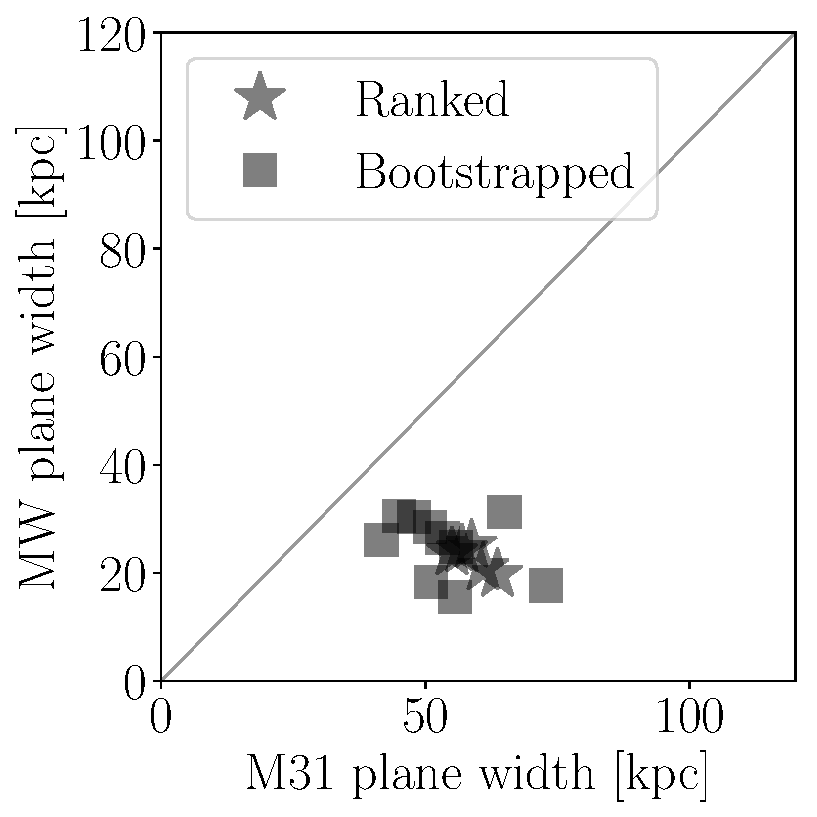
\includegraphics[width=0.40\textwidth]{LG_scatter_width.pdf}
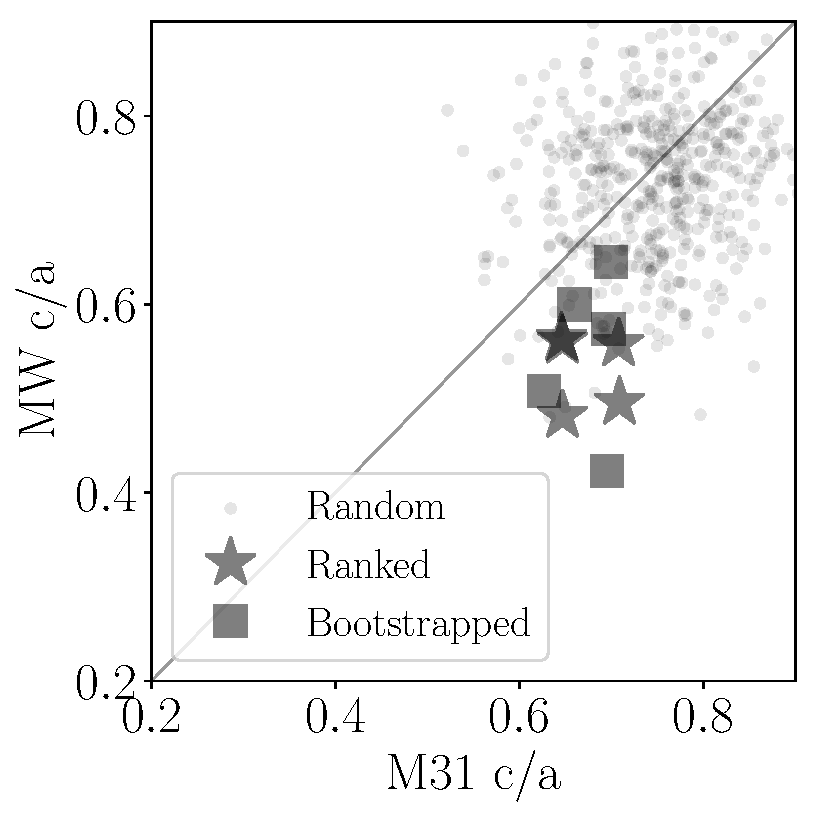
\includegraphics[width=0.40\textwidth]{LG_scatter_ca_ratio.pdf}
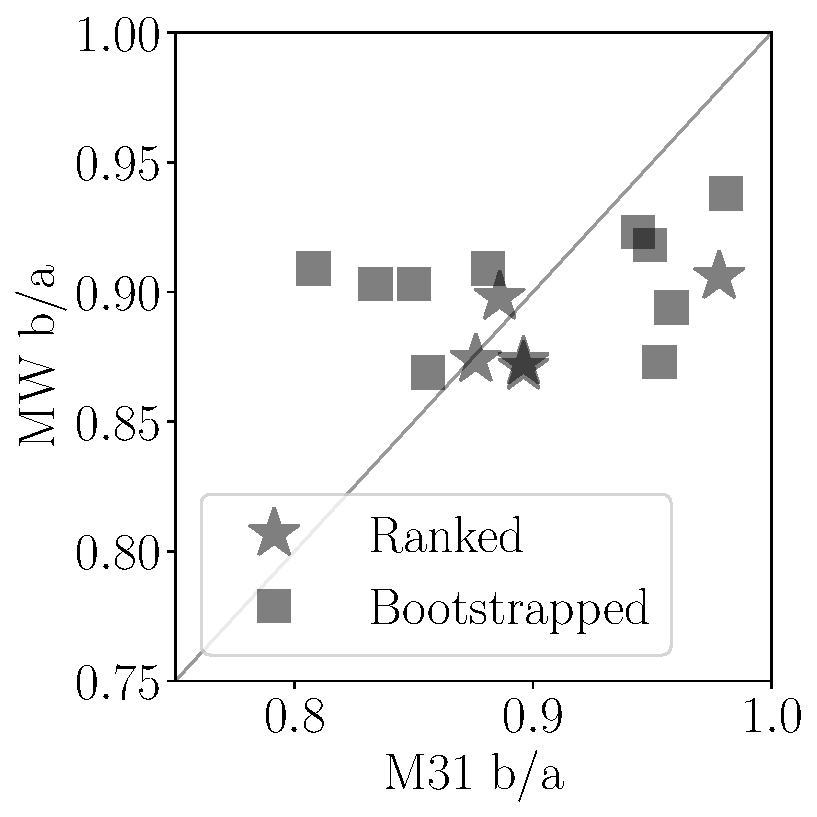
\includegraphics[width=0.40\textwidth]{LG_scatter_ba_ratio.pdf}
\caption{Basic characteristics for the MW and M31 satellite systems
\label{fig:lg_scatter}}
\end{figure*}


\begin{figure*}
\centering
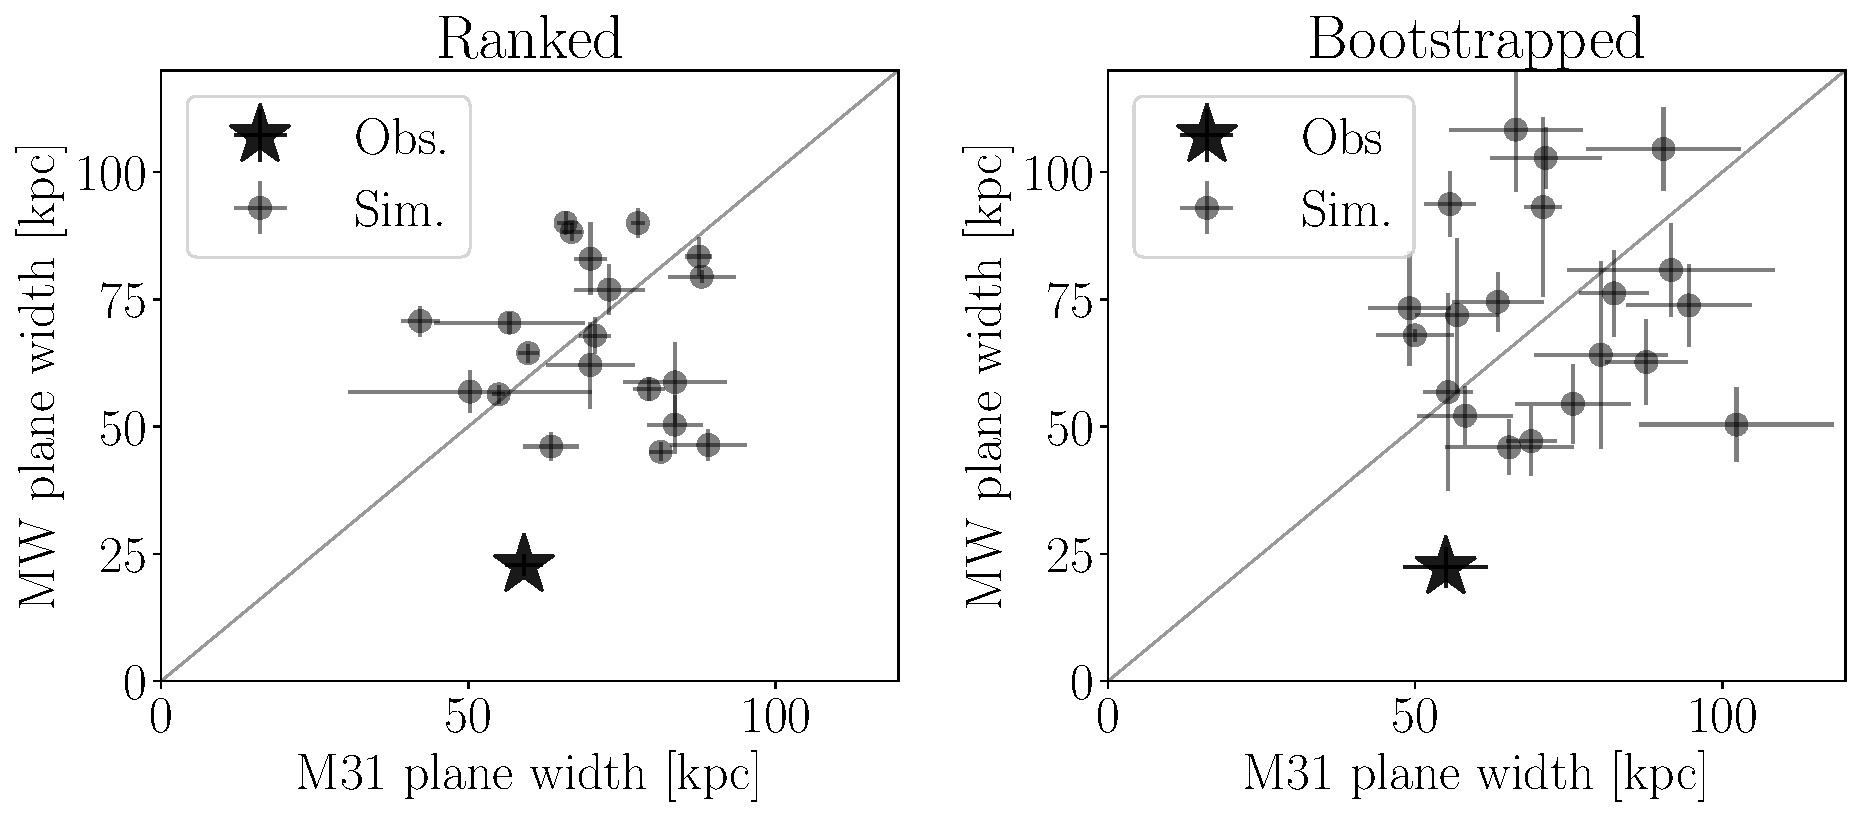
\includegraphics[width=0.7\textwidth]{scatter_width.pdf}
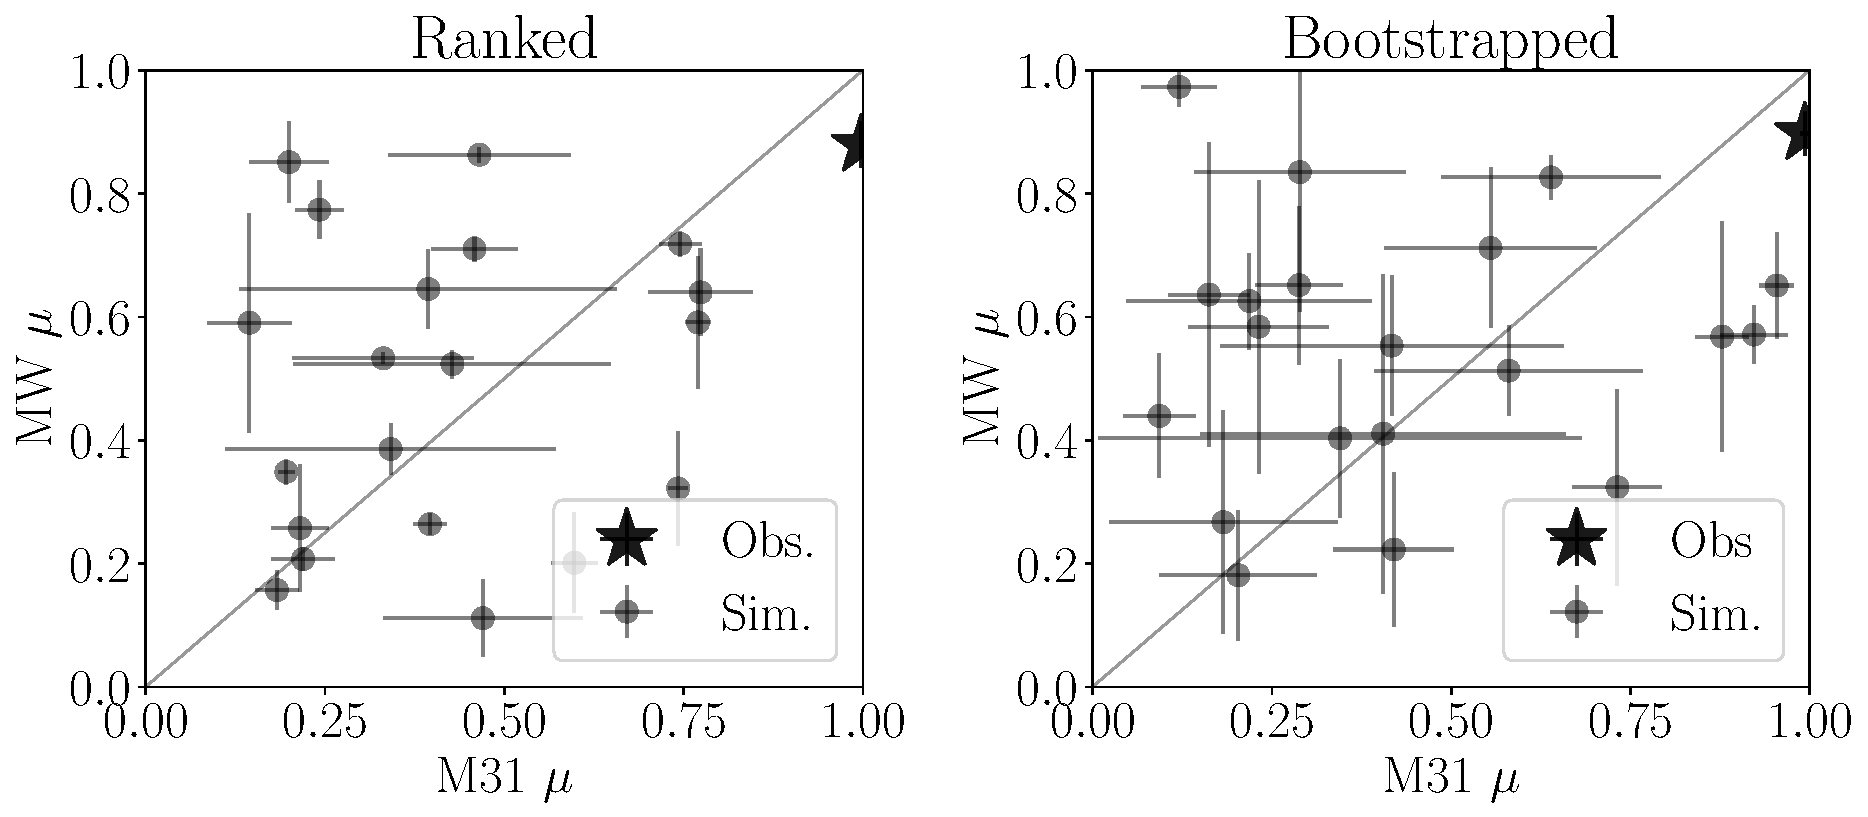
\includegraphics[width=0.7\textwidth]{scatter_mu.pdf}
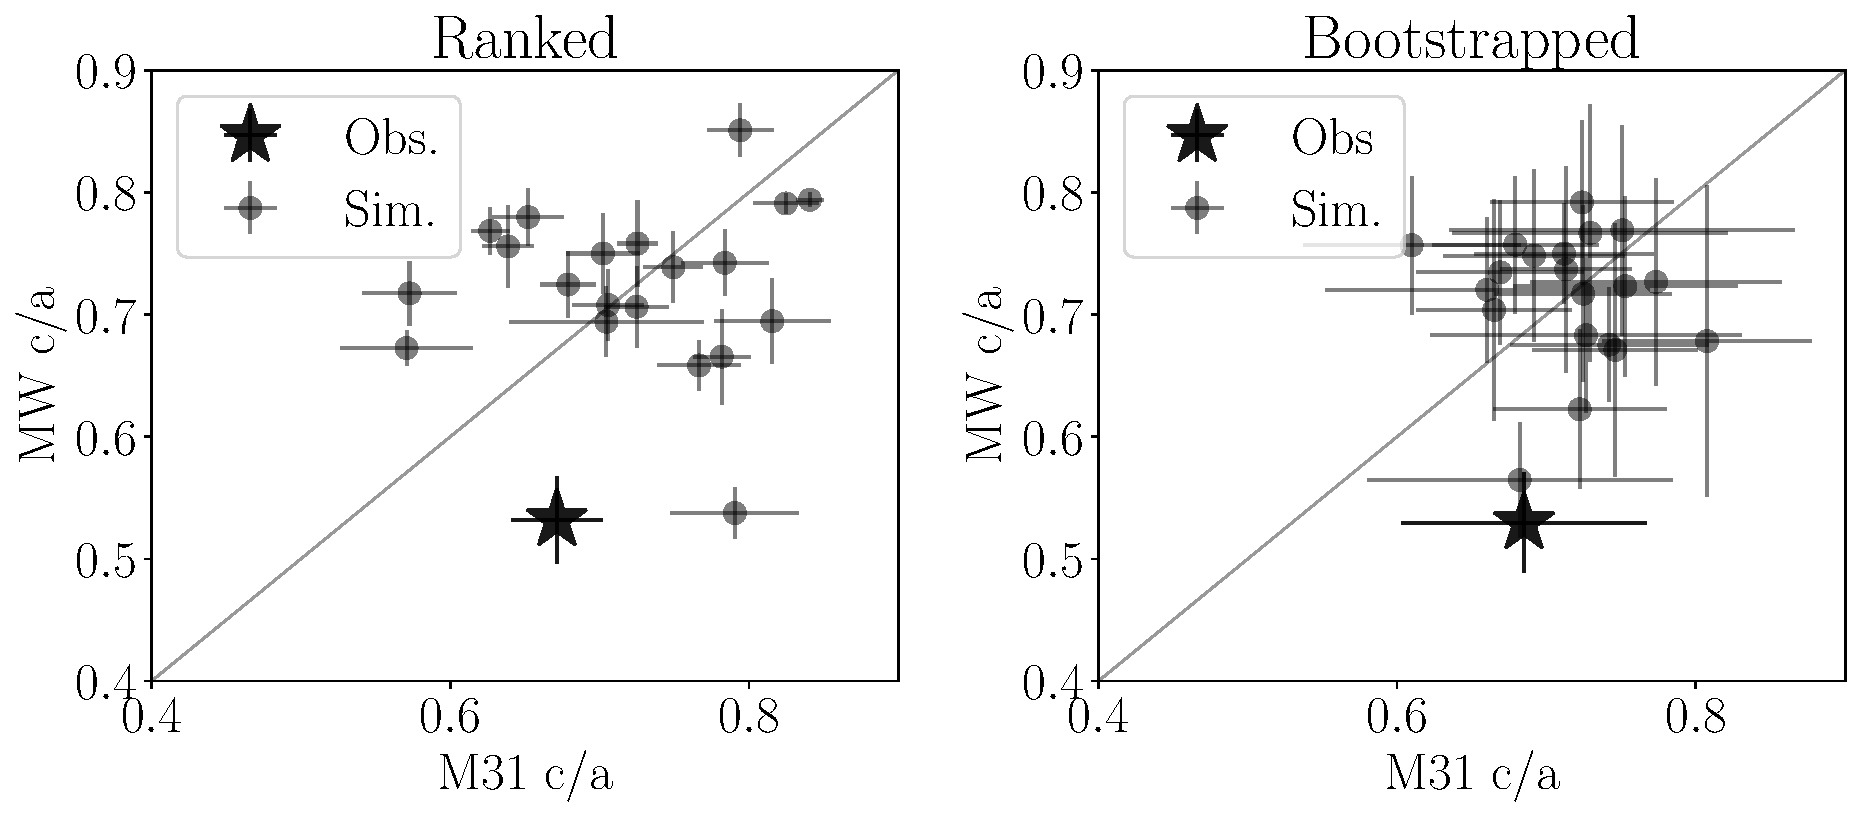
\includegraphics[width=0.7\textwidth]{scatter_ca_ratio.pdf}
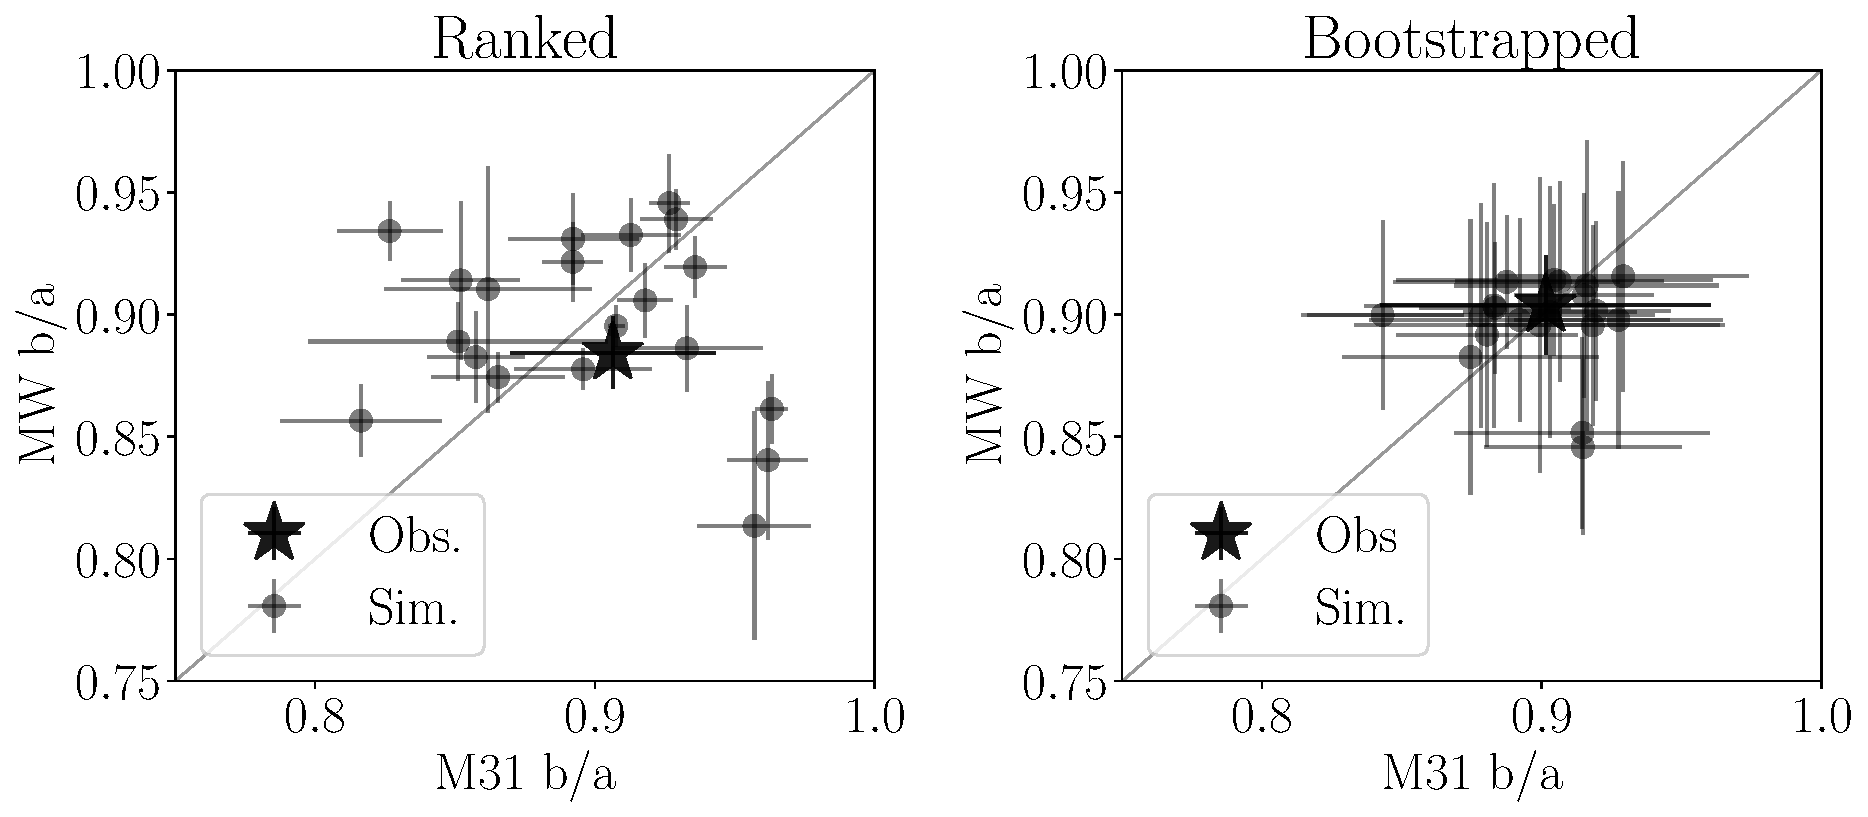
\includegraphics[width=0.7\textwidth]{scatter_ba_ratio.pdf}
\caption{Basic characteristics for the MW and M31 satellite systems
\label{fig:general}}
\end{figure*}



\begin{figure*}
\centering
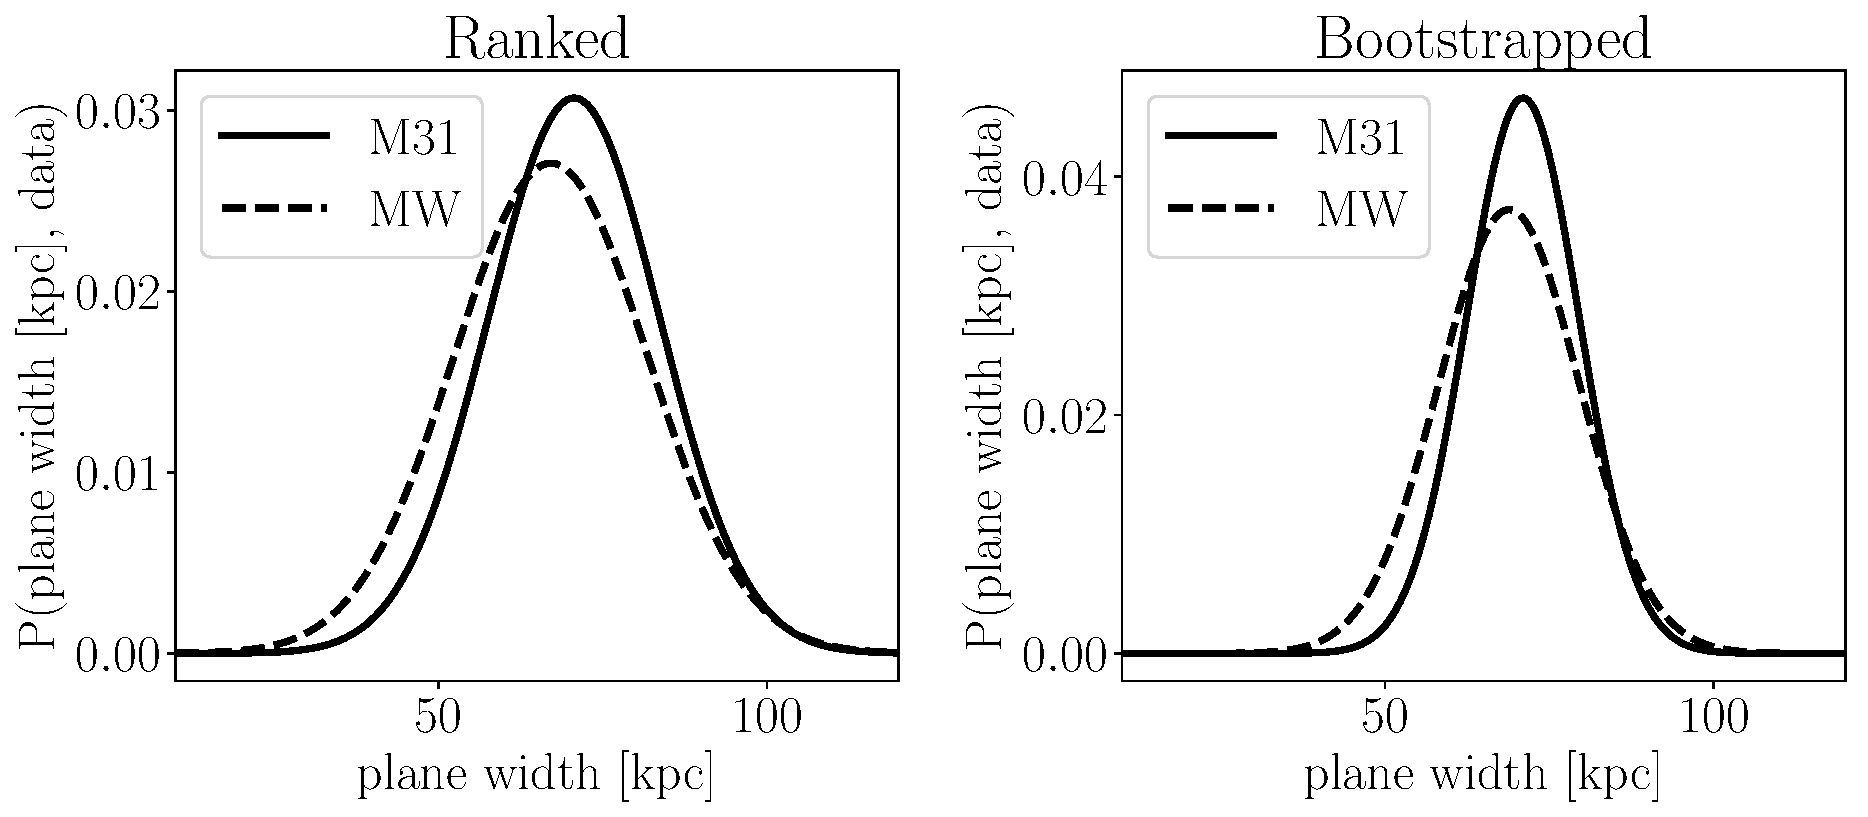
\includegraphics[width=0.7\textwidth]{distribution_width.pdf}
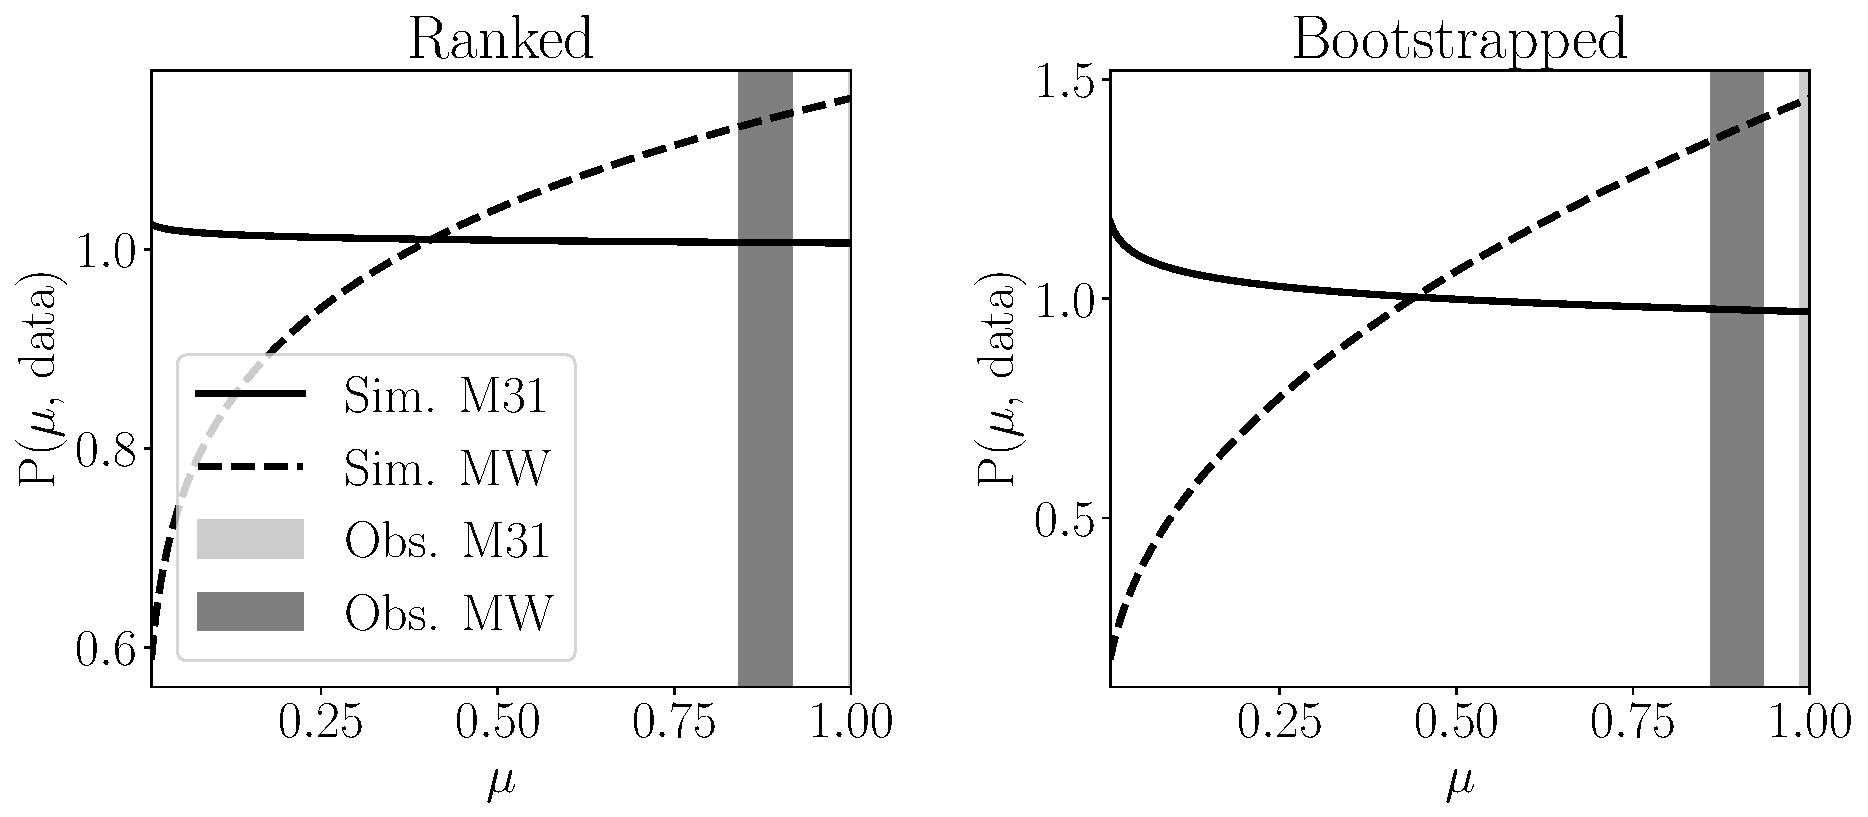
\includegraphics[width=0.7\textwidth]{distribution_mu.pdf}
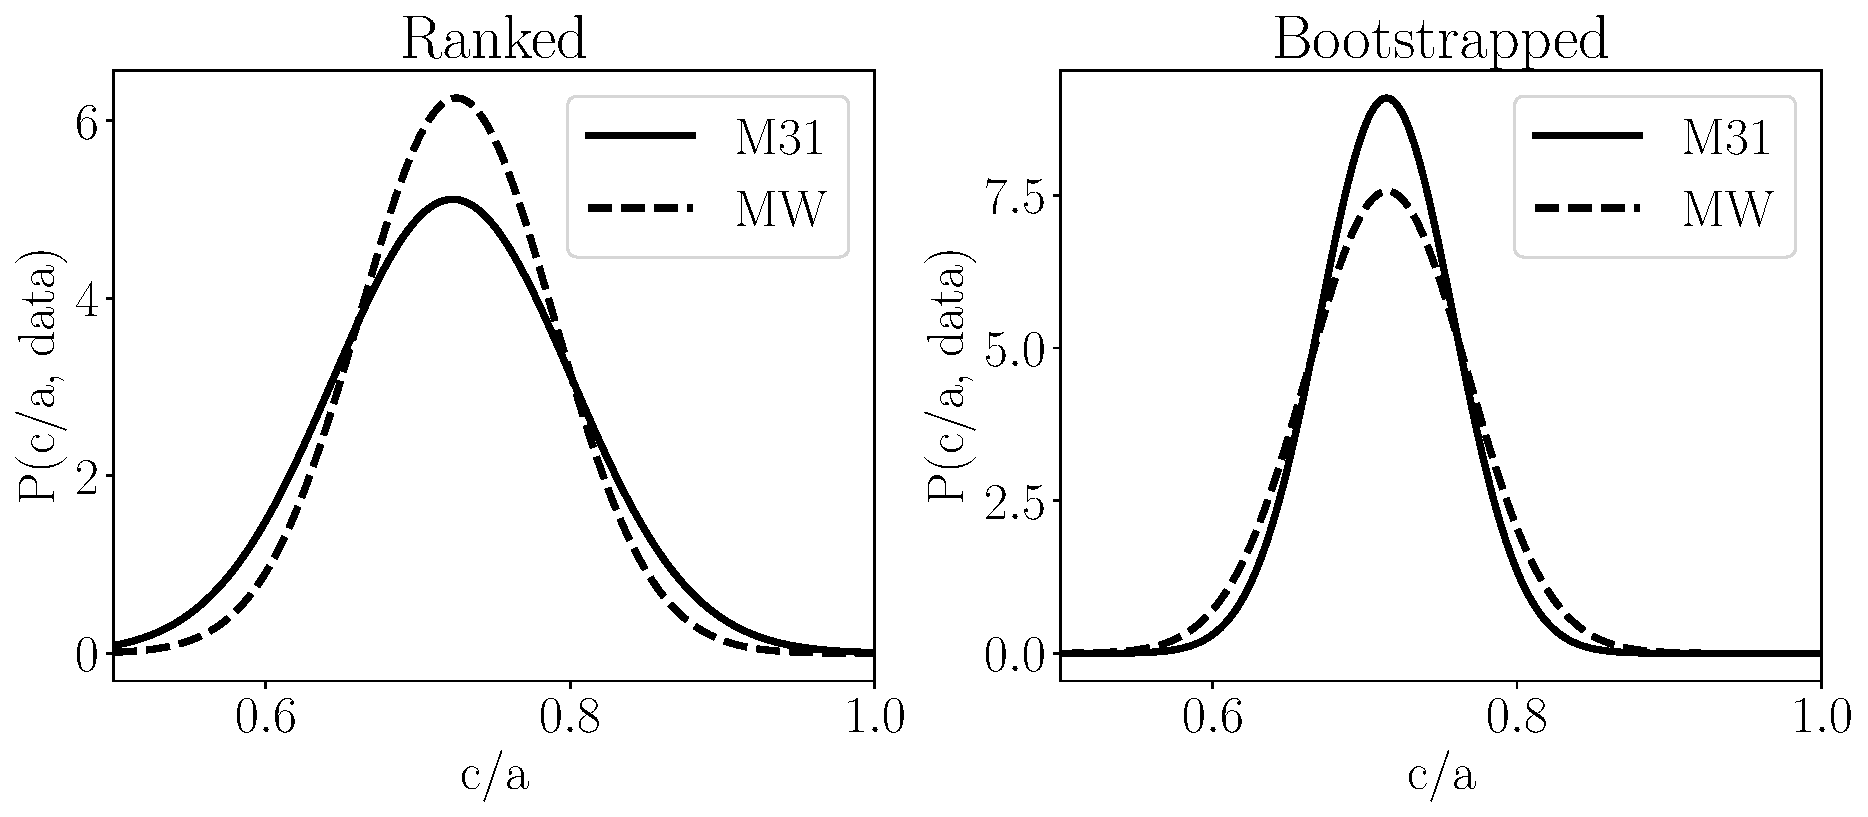
\includegraphics[width=0.7\textwidth]{distribution_ca_ratio.pdf}
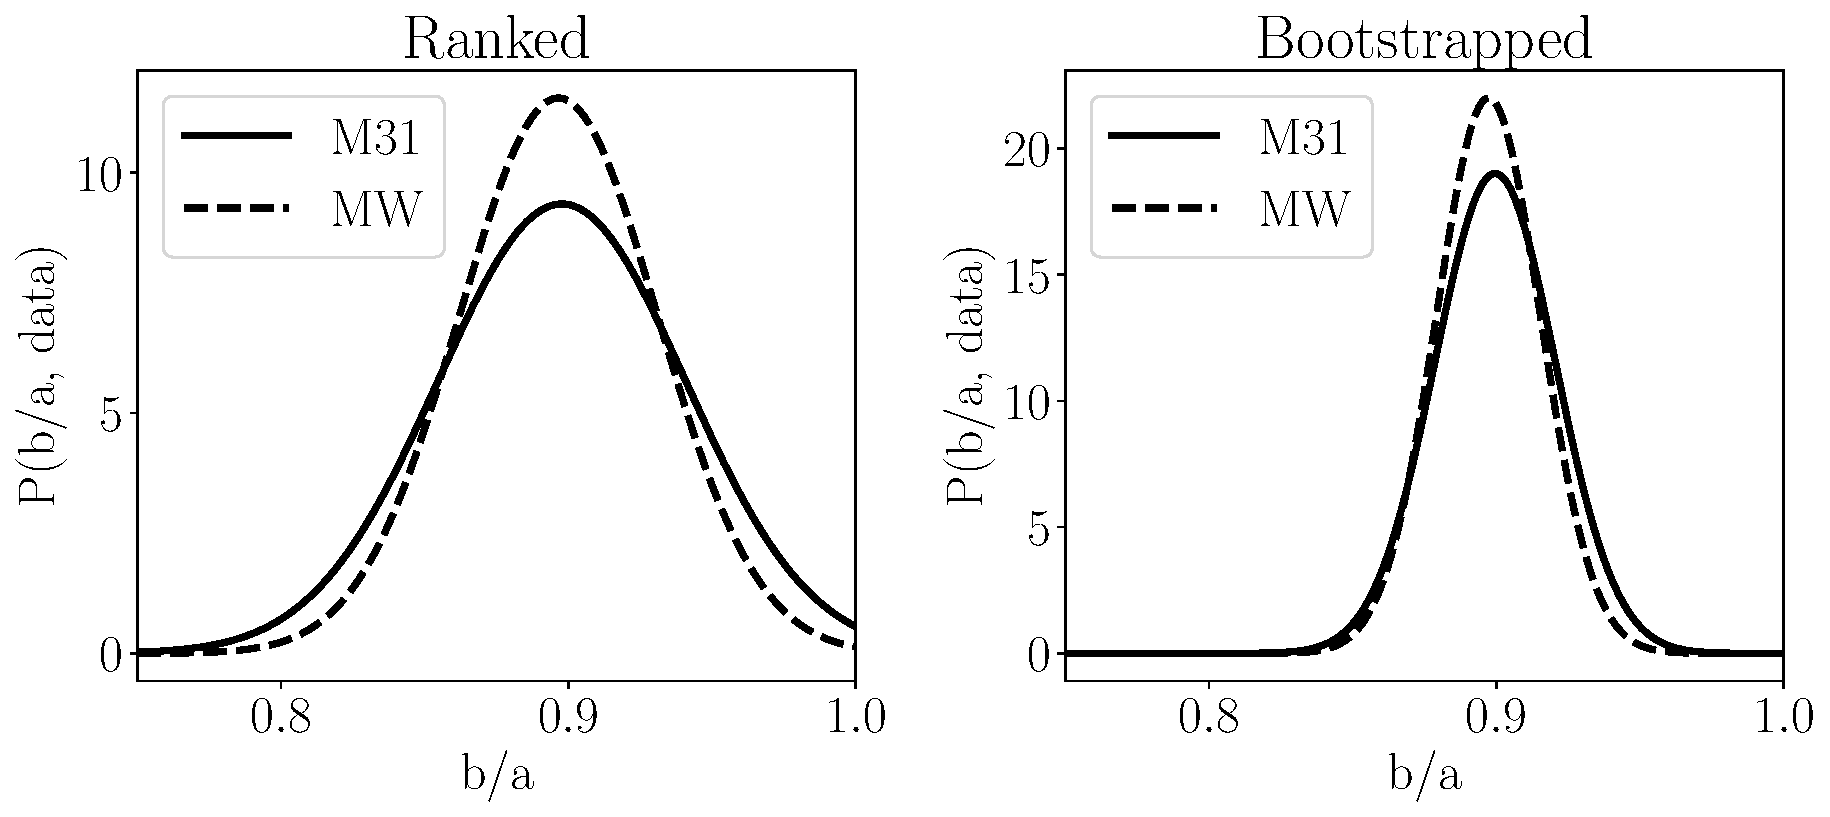
\includegraphics[width=0.7\textwidth]{distribution_ba_ratio.pdf}
\caption{Basic characteristics for the MW and M31 satellite systems
\label{fig:general}}
\end{figure*}



\section{Results}
\label{sec:results}


\subsection{Distributions in the Local Group}

Figure \ref{fig:lg_scatter} summarizes our main results for the
observed LG satellite distributions.
In all panels the diagonal line corresponds to the 1:1 ratio.

Here we can see that the mean values of the \texttt{Ranked} and
\texttt{Bootstrapped} samples are similar within the scatter in each
sample. 
The scatter is itself tends to be larger in the \texttt{Bootstrapped}
sample. 
This allows to stablish the LG uncertainties to be used in the next
sections to compare it against the distributions derived from the
Illustris simulation.

There is a third sample in Figure \ref{fig:lg_scatter}. 
It corresponds to the set of \texttt{Random} points that were generated
by randomizing the angular positions of the satellites in the
\texttt{Bootstrapped} samples. 
This allows us to understand the importance of intrinsic satellite's
radial profile distribution in driving the results.  





\begin{table*}
  \centering
\begin{tabular}{lll}
\hline\hline
Symbol & Units & Description\\\hline
$\hat{r}_{AB}$& & Unit vector along the direction connecting two
dominant galaxies\\
$N_s$ & & Number of satellites\\
$a > b> c$ & kpc & Inertia tensor eigenvalues. \\
$\hat{I}_1$, $\hat{I}_2$, $\hat{I}_3$ & & Inertia tensor eigenvectors. \\
$\sigma_s$ & kpc & Ellipsoid width\\
\hline\hline
\end{tabular}
  \caption{Overview of the parameters computed for each central galaxy
    and its satellite system.
  \label{tab:models}}
\end{table*}



\bibliographystyle{mnras}
\bibliography{Dwarfs}

%% Alignments between galaxies, satellite systems and haloes
%% https://arxiv.org/pdf/1605.01728.pdf

%M31 mass
%% https://arxiv.org/abs/1410.0017

%MW mass
%https://arxiv.org/abs/1407.1078


\end{document}

